\chapter{大动态范围读出方案的设计与验证}
\label{ch:large_dynmaicrange}
一个探测器本征的探测性能由其构型和使用的探测介质材料决定。
探测器的本征分辨是相对固定的,在研制阶段,一般通过物理过程的蒙卡模拟(如Geant4)对其进行研究。
探测器实际的探测性能还取决于其读出设计,包括读出器件的选择、读出方案以及前端电子学的设计。
探测器的读出设计相对灵活,往往需要针对探测器的功能需求进行特殊设计,在研制阶段,一般经过多次的‘设计-实验验证’循环来确定最佳的设计方案。
合理的读出设计可以将探测器的本征探测性能发挥到极致,这也是探测器研制的主要目标。

对于PSD来说,它首先需要覆盖质子数$Z=1 \sim 20$的重离子探测。
根据第二章的描述(见\ref{sec:description:psd_principle}节),相对论重离子在PSD塑闪单元条中的沉积能量近似正比于$Z^2$。因此,不同种类带电粒子在PSD中的输出信号幅度变化范围巨大,这对PSD探测单元模块读出方案的动态范围提出了上限要求。
另一方面,PSD同时需要对高能$\gamma$和高能$e$进行鉴别,即通过信号的有/无来判断入射粒子是否带电(见\ref{sec:description:psd_principle})。
为了降低$e/\gamma$误判率,PSD探测单元模块的读出方案需要足够敏感,能够有效区分带电粒子信号与电子学基线噪声信号,
这对其动态范围提出了下限要求。
一般的读出设计不能同时满足上述两方面的需求,我们需要对PSD探测单元模块的读出进行特殊设计,以满足其大动态范围的要求。

本章对PSD的读出方案设计进行了详细的论述,主要包括以下内容:PSD动态范围需求的估算,PSD读出方案的详细设计流程以及PSD大动态范围读出方案的实验验证。


\section{重离子在塑料闪烁体中的光产额}
\label{sec:dynamic_range:light_yield}
PSD使用PMT作为读出器件,因此入射粒子在塑料闪烁体中的闪烁光输出多少直接影响其输出信号的幅度。
在沉积能量密度不大的条件下,闪烁光输出与入射粒子的沉积能量大小成正比。
这种情况较为简单,我们可以通过对沉积能量大小的估算直接推出闪烁光输出的幅度范围。
但对于重离子来说,它们在物质中的沉积能量密度较大,此时猝灭效应\cite{birks_book_2013}(quenching effect)的影响显著。
因此,重离子引起的闪烁光输出与沉积能量大小不成正比关系,我们需要研究它们在塑料闪烁体中的光产额差异大小,为PSD动态范围需求的估算提供基础。

当带电粒子或$\gamma$射线入射到闪烁体内,使得闪烁体内的原子(分子)电离、激发,在退激过程中发光,这就是闪烁体发光的基本原理。
退激过程也可以不通过发射荧光光子的形式进行,而以其它形式将退激放出的能量转化为热能输出,这就是猝灭效应。
它使得闪烁体的发光量减少,并最终趋于饱和(saturation)。
猝灭效应与原初电离密度有关,电离密度越高,猝灭效应就越强,光响应偏离线性的程度也就越大。
闪烁体的猝灭效应一般用Birks定律进行描述\cite{birks_article_1951}:
\begin{equation}
	\frac{dL}{dx} = \frac{SdE/dx}{1+kBdE/dx}
	\label{eq:dynamic_range:birks_law_dE}
\end{equation}
其中$dL/dx$是单位路径的闪烁光产额,$dE/dx$是入射粒子的单位路径能量损失,$S$是发光效率(scintillation efficiency),$k$是猝灭因子,代表沉积能量中产生猝灭效应的比例,而$B$是一个常数。$kB$经常合在一起,被称为Birks系数。
当$dE/dx$较小时,猝灭效应并不明显,公式\ref{eq:dynamic_range:birks_law_dE}变为$dL/dx \approx AdE/dx$,即光产额与沉积能量成正比;当$dE/dx$很大时,公式\ref{eq:dynamic_range:birks_law_dE}变为$dL/dx \approx A/k_B$,即光产额近似是个常数,与沉积能量的大小无关,这就是猝灭效应导致的光饱和现象。
由于PSD只需对入射重离子的电荷量进行测量,我们希望得到塑闪光产额与入射粒子质子数$Z$(宇宙线重离子的核外电子都是完全剥离的,因此它们的电荷数就是质子数)的关系。
对于相对论重离子穿过薄的探测介质,$dE/dx \propto Z^2$。将这个关系带入到公式\ref{eq:dynamic_range:birks_law_dE},可到得到
\begin{equation}
	\frac{dL}{dx} = \frac{S' Z^2}{1+{k'}{B'} Z^2}
	\label{eq:dynamic_range:birks_law_Z}
\end{equation}
上式就是Birks定律应用到PSD中的结果。
在后面的论述中,我们都将使用$Z^2$来表述闪烁体光产额对入射粒子种类的依赖关系。

闪烁体的发光机制非常复杂,并没有统一的理论框架可以对其进行完备的描述。
公式\ref{eq:dynamic_range:birks_law_Z}只是一个半经验公式,其中的参数$S$和Birks系数虽然具有明确的物理意义,但一般需要通过对实验数据进行拟合得到。
而且,它们的具体数值与入射的粒子种类有关,这反应了猝灭效应的粒子种类关联性(particle-species dependence)。
另一方面,上述简单形式的Birks定律只能够描述闪烁体对低能入射粒子的光响应,当入射粒子能量升高到相对论能区时,就需要对Birks定律进行扩展。
相对论能区的光响应还有另外一个特点:那就是猝灭效应与入射粒子种类的关联性减弱,光产额主要取决于沉积能量大小\cite{matsufuji_response_1999}。
因此,Birks定律以及以下所有Birks定律的拓展形式中的自由参数具有普适性,即它们的值与入射粒子种类无关。

一种常见的扩展形式是在Birks定律的分母中加入$dE/dx$的二次项,即
\begin{equation}
	\frac{dL}{dx} = \frac{S' Z^2}{1+k'B'Z^2+C'Z^4}
	\label{eq:dynamic_range:birks_chou_law}
\end{equation}
其中$C'$是常数。这种扩展形式是Chou首次提出\cite{chou_nature_1952},因此上式被称为Birks-Chou公式。
另一种常见的扩展形式是基于闪烁体发光的BTV模型\cite{voltz_influence_1966,tarle_cosmic_1979}(Birks-Tarle-Voltz model,简称BTV模型)。该模型认为闪烁光按其产生的区域,可以被分为两部分“core”和“halo”两部分。
core区域在入射粒子的径迹附近,这里是电离过程发生的主要区域,分布有大量电离产生的低能电子;halo区域分布在core的外围,它由电离产生的少量高能$\delta$电子逃离core区域后形成。core区域内的电离密度较高,因此猝灭效应显著,该区域的光响应可以用Birks定律描述;halo区域的电离密度较低,猝灭效应可以忽略,该区域的光响应与沉积能量成正比。
假设halo区域的沉积能量占总沉积能量的比例为$F_s$,则基于BTV模型拓展的Birks定律可以表示为
\begin{equation}
	\frac{dL}{dx} = S(\frac{(1-F_s)Z^2}{1+B_s(1-F_s)Z^2}+F_sZ^2)
	\label{eq:dynamic_range:btv_law}
\end{equation}
其中$S$是一个常数,$B_s$表征猝灭效应强度的一个量。
除了这两种常见的扩展方式外,还有其它不较常使用的扩展形式,如Wright提出的\cite{wright_scintillation_1953}
\begin{equation}
	\frac{dL}{dx} = A \ln(1+aZ^2)
	\label{eq:dynamic_range:wright_law}
\end{equation}
其中$A$和$a$都是常数。
所有这些对Birks定律的扩展,它们的行为在$dE/dx$较小时都是一致的(即正比于光产额正比于沉积能量大小);但当$dE/dx$较大时,不同形式的扩展给出的结果相差很大。
虽然各种扩展形式在特定条件下,都可以准确地描述已有的实验数据点,但它们各有各的局限性,都不适合作为“第一性原理”来估算不同的相对论重离子在PSD塑闪条中的光产额差异。

\begin{figure}[htbp]
	\centering
	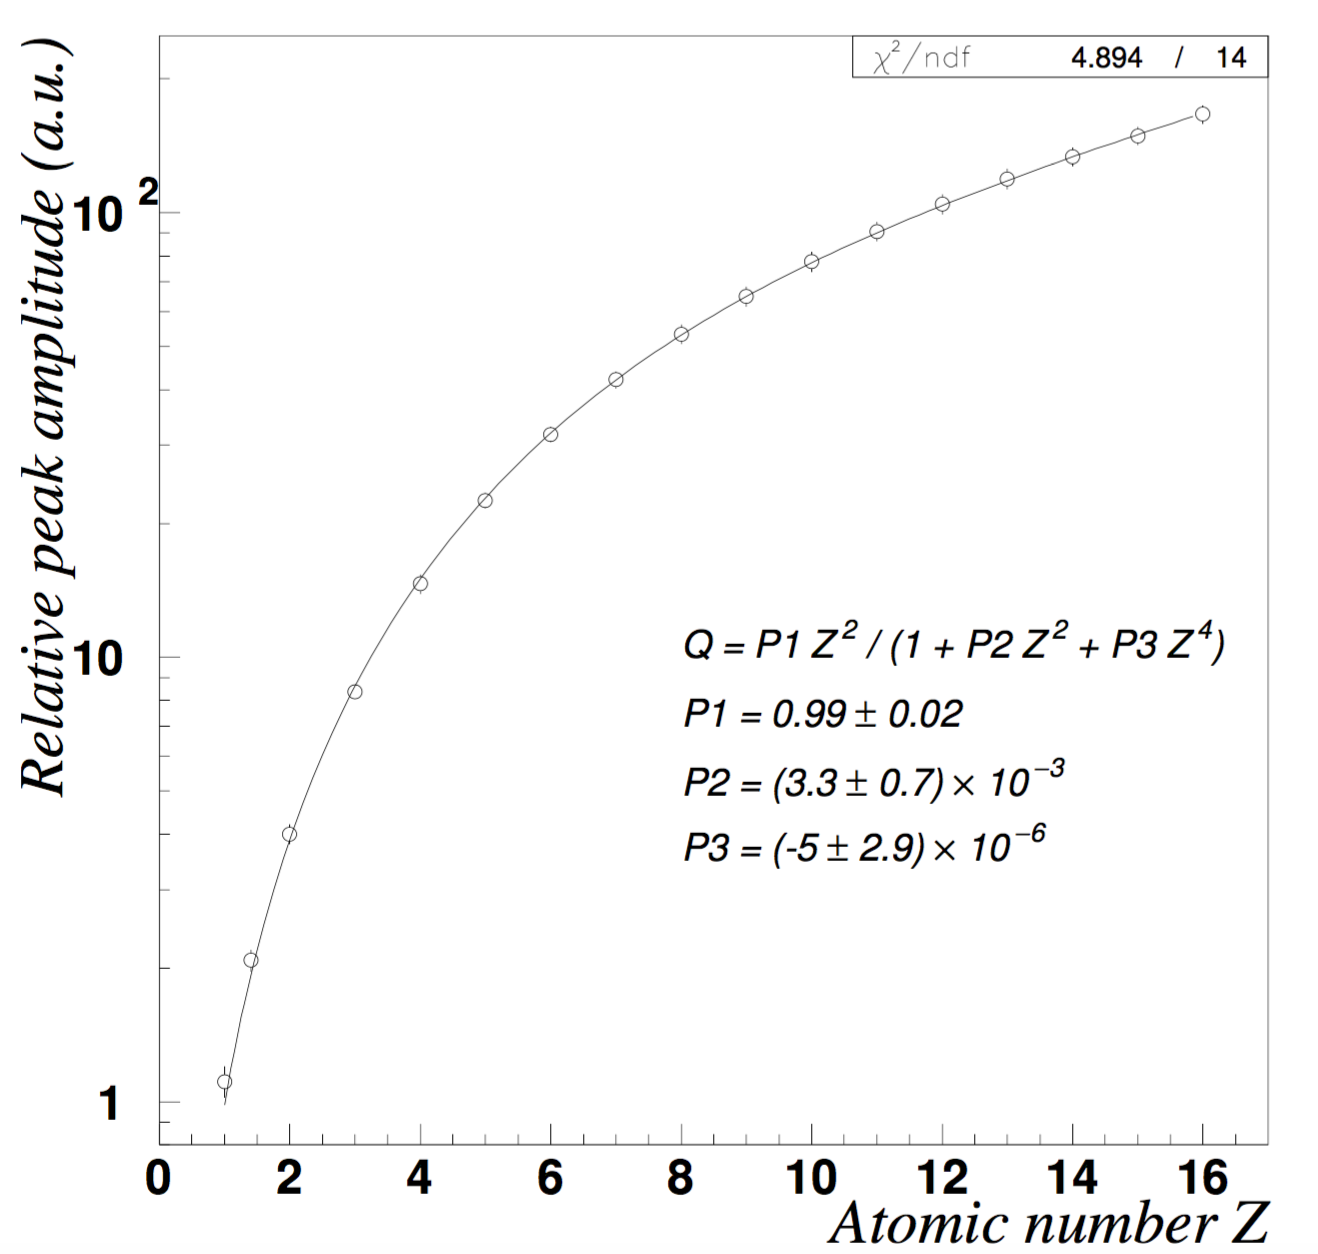
\includegraphics[width=0.6\textwidth]{chap/dynamic_range/fig/ams02_tof.png}
	\caption{AMS02-TOF得到的光响应曲线,横轴为质子数,纵轴为相对光产额。图中的圆点是实验数据点,实线是利用公式\ref{eq:dynamic_range:birks_chou_law}对数据点的拟合结果。}
	\label{fig:dynamic_range:AMS02}
\end{figure}

由于理论模型的局限性,我们基于AMS02-TOF束流测试的实验结果\cite{bindi_performance_2005}来得到相对论重离子在PSD塑闪条中的光产额差异。
束流测试在CERN的SPS进行,通过主束轰击Be靶得到不同种类的次级离子,主束使用的是\SI{20}{AGeV/c}和\SI{158}{AGeV/c}的Pb。
由于AMS02-TOF使用的探测介质与PSD完全一致,都是\SI{10}{mm}的EJ-200,该实验结果可以直接被PSD参考和使用。
图~\ref{fig:dynamic_range:AMS02}给出了AMS02-TOF得到的光响应曲线,数据点从$Z=1\sim16$。
使用扩展公式\ref{eq:dynamic_range:birks_chou_law}可以准确地拟合实验数据点,得到的拟合参数值为$S'=0.99(0.02)$,$k'B'=3.3(0.7)\times10^{-3}$,$C'=-5(2.9)\times10^{-6}$。
根据拟合结果,可以外推得到$Z=20$时的相对光产额,约为$Z=1$时的270倍。
该结果是我们估算PSD动态范围需求的基础。



\section{PSD动态范围需求的估算}
\label{sec:dynamic_range:estimation}
闪烁体的实际发光量不仅与其光响应有关,而且还与入射粒子穿过的厚度和能量涨落有关。
另外,PSD输出信号的大小直接决定于单元条端头PMT接收到的光子数,因此最终的动态范围还会受到光在单元条中传输导致的衰减效应的影响。
本节结合这些因素,对PSD的动态范围做了一个合理的估算,该估算结果被用于指导PSD探测单元模块大动态范围读出方案的设计。

在高能粒子探测器领域,设计人员经常使用最小电离粒子(Minimum Ionizing Particle,简称MIP)来对探测器进行测试和刻度。
对于PSD覆盖的相对论能区,所有的被测粒子(质子,重离子,电子)的能量都在Beth-Block曲线的费米坪区内,它们的电离能损与最小电离值相差不大,因此它们在本文中也可以被称为MIP粒子。
为了叙述的方便,我们将单电荷的最小电离粒子垂直穿过PSD塑闪单元条中心时端头PMT接收到的光输出量定义为\SI{1}{MIP},并以它为单位来表述PSD的动态范围需求。
由上节的结果可以看到,不同入射重离子在PSD塑闪条中的光产额最大相差270倍。
所有单电荷(singly charged)的MIP粒子在PSD单元条中都有相同的沉积能量,这也意味着它们有相同的光产额,因此上述结果可以拓展到所有带电粒子,即不同种类带电粒子在PSD塑闪单元条中的光产额为\SI{1}{MIP}$\sim$\SI{270}{MIPs}。

入射粒子在闪烁体中穿过的距离越大,它在物质中的能量沉积也就越大,产生的闪烁光子数也就越多。
对于PSD单元条这样厚度薄、密度小的探测介质,入射粒子在其中的单位路径能量损失率$dE/dx$以及单位路径的光产额$dL/dx$可以近似认为是个常数,这意味着能损大小以及光产额与入射粒子穿过的路径成正比。
DAMPE探测器设计有较大的视角,需要覆盖的入射角度为$[\SI{-60}{\degree},\SI{60}{\degree}]$。
这意味着入射粒子在PSD单元条中穿过的最长距离是垂直入射时的两倍。
因此,带电粒子在PSD中的光产额上限被扩展到\SI{540}{MIPs}。

上面讨论的都是平均光产额,而入射粒子在闪烁体中的能量损失过程和闪烁体的发光过程在本质上都是随机过程,这会带来光输出量的统计涨落。
实际的光输出量服从高斯分布,其中心值是平均光产额,标准偏差即探测介质的本征分辨率。
假设EJ-200的能量分辨率为\SI{10}{\percent},并且认为$5\sigma$可以覆盖整个高斯分布,则PSD单元条光产额的上限就扩展到\SI{675}{MIPs},而下限被减低到\SI{0.75}{MIPs}。

闪烁光子在入射粒子的击中位置处产生,它们需要在单元条内经过一系列的反射、折射和吸收过程,才能传输到端头,最终被PMT接收。
部分闪烁光子会在传输过程中损失掉,且传输的距离越长,损失的光子数越多。
为了尽量减少闪烁光长距离传输造成的衰减,PSD塑闪单元条进行了表面抛光,并且外部紧密包裹了一层高反射率的Tyvek纸以提高反射效率。
由于PSD单元条长度很长,上述措施并不能把光的传输衰减完全消除掉,这使得相同入射粒子在不同击中位置处产生的输出信号幅度并不一致。
该现象被称为光收集不均匀性,它极大地扩展了PSD输出信号的动态范围。
初步测试显示,从PSD单元条中心到单元条最远端的光衰减比例以及从单元条最近端到单元条中心的光衰减比例都可以被有效控制在\SI{50}{\percent}以上。
因此,PSD端头PMT接收到的闪烁光强度在应该在\SI{0.375}{MIPs}到\SI{1350}{MIPs}之间。

最后,为了将带电粒子产生的最小信号与电子学基线的噪声信号有效区分开来,同时适当预留部分动态范围供调节使用,PSD的动态范围需求被确定为$\SI{0.1}{MIPs}\sim\SI{1400}{MIPs}$。

\section{大动态范围读出方案的设计}
\label{sec:dynamic_range:design}

\subsection{设计思路}
\label{sec:dynamic_range:readout_scheme}
PSD使用ASIC芯片VA160进行电荷测量。该芯片集成了32个输入通道,每个通道的动态范围为$\SI{-3}{\pico\coulomb}\sim\SI{13}{\pico\coulomb}$(详见第\ref{ch:description}章)。显然,单个VA160通道不能够覆盖所需的动态范围。因此,PSD探测单元模块采用了下述的读出设计:以双打拿极引出的方式,从单个PMT得到两路不同增益的输出信号,然后将两路信号分别输入到不同的VA160的测量通道中。当光输出量较小时,可以使用低增益的通道进行测量;当光输出量较大时,此时低增益通道已经饱和,可以使用高增益的通道进行测量。同时,为了降低高增益通道对低增益通道的干扰,高增益通道的信号和低增益通道的信号被输出到不同的VA160芯片中,如图~\ref{fig:dynamic_range:readout_scheme}所示。

\begin{figure}[!htb]
	\centering
	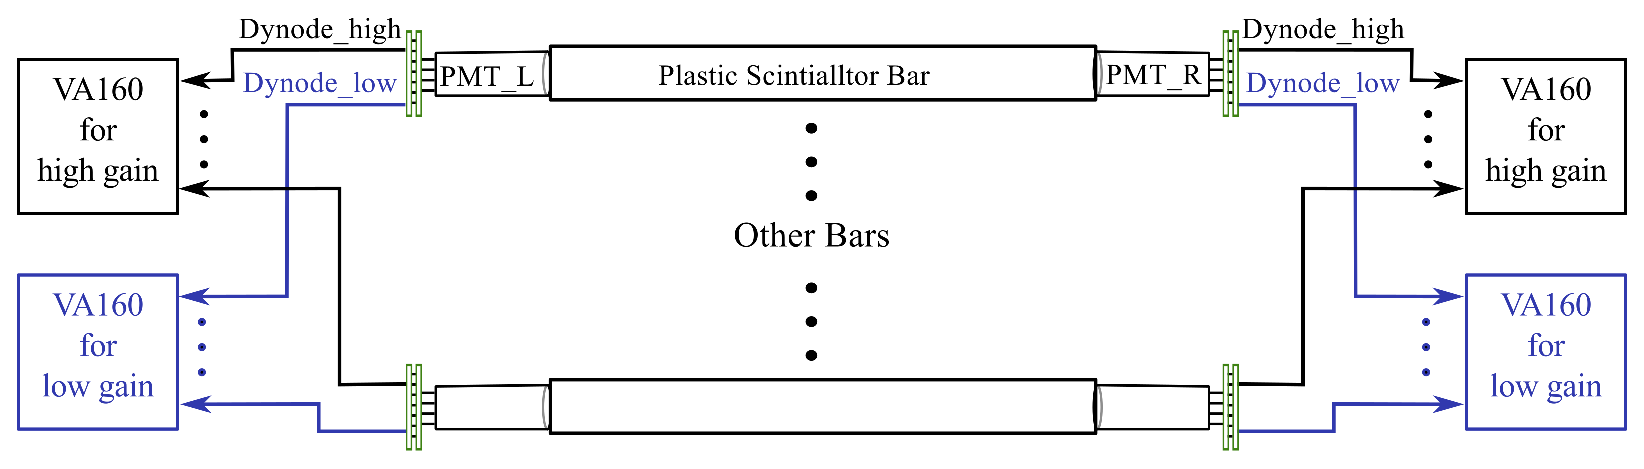
\includegraphics[width=\textwidth]{chap/dynamic_range/fig/readout_scheme.eps}
	\caption{PSD探测单元模块的读出方案}
	\label{fig:dynamic_range:readout_scheme}
\end{figure}

中国科学院近代物理研究所基于VA160芯片开发了PSD的前端电子学模块(Front-End Electronic,简称FEE),详见第\ref{ch:description}章。
测试显示,该FEE模块的有效线性范围为$\SI{0}{\pico\coulomb}\sim\SI{12}{\pico\coulomb}$,且每个测量通道的电子学噪声可以控制在\SI{6}{\femto\coulomb}内~\ref{fig:dynamic_range:fee_test}。
假设最少需要$5\sigma$的分离度来区分真实信号与基线噪声,这意味着PSD读出电子学对\SI{0.1}{MIPs}的测量值应该大于\SI{30}{\femto\coulomb},即$\SI{1}{MIP} \ge \SI{300}{\femto\coulomb}$。
因此,高增益打拿级对应通道的动态范围应该覆盖$\SI{0.1}{MIPs}\sim\SI{40}{MIPs}$余下的动态范围由低增益打拿级对应的通道覆盖,这限制了两个打拿级间的增益系数必须$\ge 35$。
这两个要求是下一节中对打拿极进行选择的依据。

\begin{figure}[!htb]
\centering
\subfloat[][FEE某通道的基线噪声谱]{
	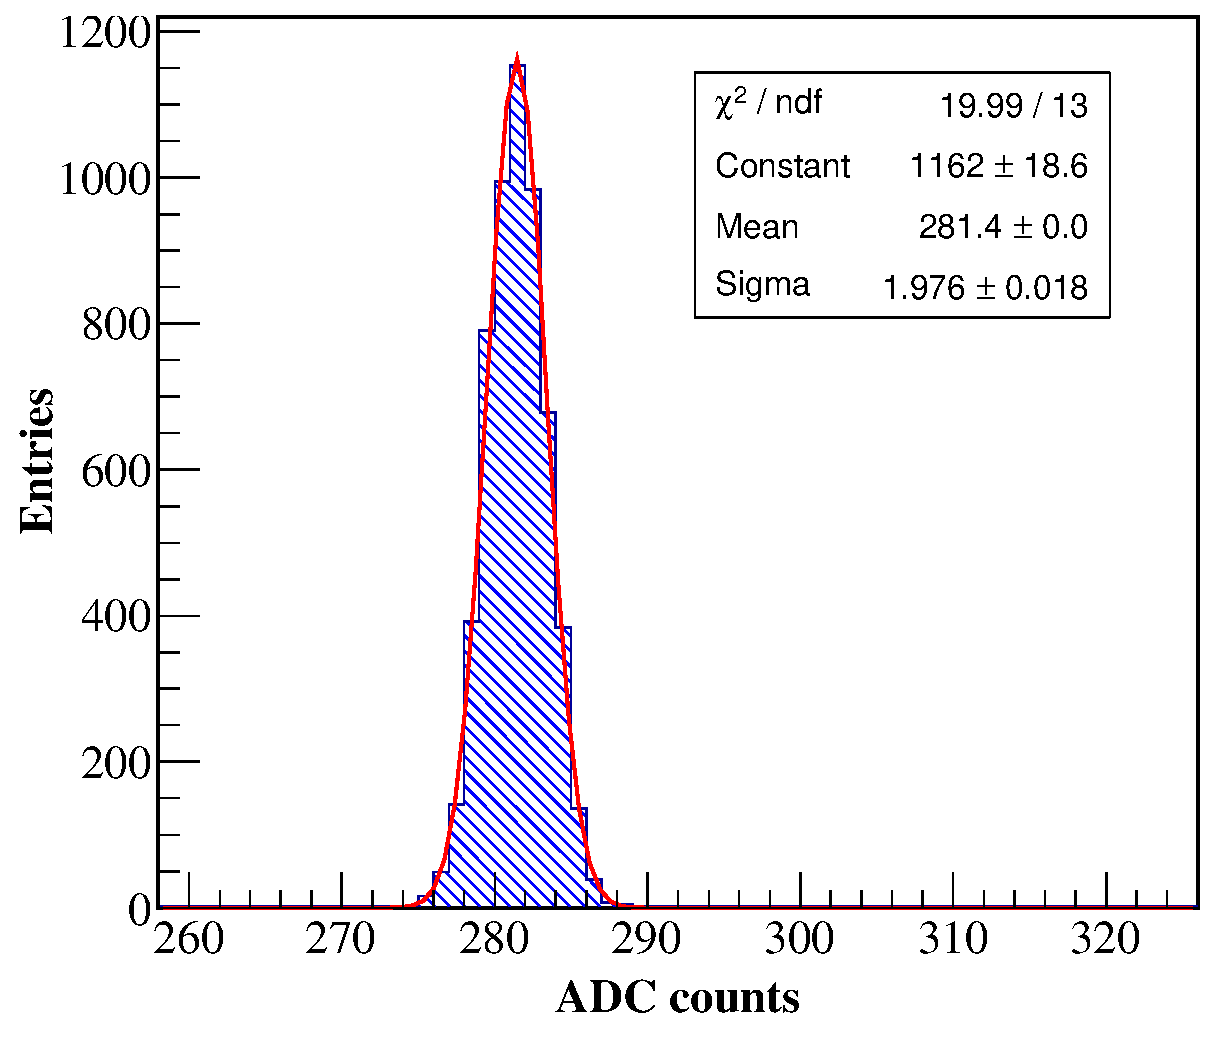
\includegraphics[width=0.48\textwidth]{chap/dynamic_range/fig/ped.eps}
}
% \hfill
\subfloat[][FEE某通道的电子学刻度结果]{
	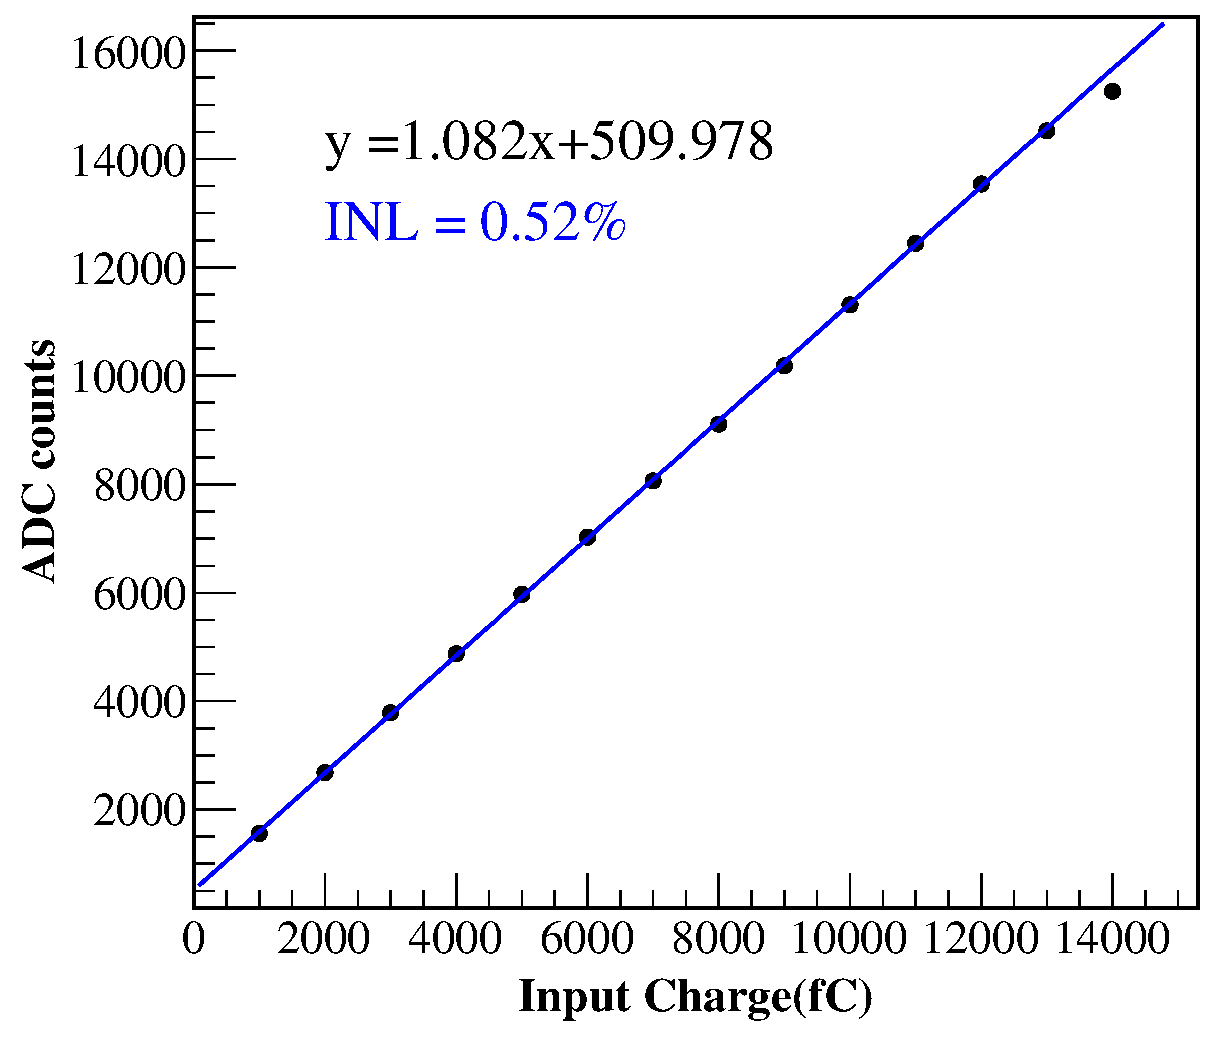
\includegraphics[width=0.48\textwidth]{chap/dynamic_range/fig/elec_calib.eps}
}
\label{fig:dynamic_range:fee_test}
\caption{FEE的测试结果}
\end{figure}

\subsection{打拿极的选择}
\label{sec:dynamic_range:dynode_selection}
PMT的不同打拿极对应不同的增益系数,而R4443具有10个打拿极级数。
为了从中选出合适的两个打拿极级数用于信号引出,需要对\SI{1}{MIP}信号产生的平均光电子数(Photoelectrons,简称PE)进行估算(这里的\SI{1}{MIP}同\ref{sec:dynamic_range:estimation}节的定义,即需要对单电荷最小电离粒子垂直穿过PSD塑闪单元条时端头PMT产生的光电子数进行估算)。
根据得到的平均光电子数值,就能进一步估算出各个打拿极输出信号的电荷量。
最终,结合上一节得到的动态范围要求和打拿极间的相对增益要求,我们就能确定合适的打拿极级数。

单电荷最小电离粒子在\SI{10}{mm}塑料闪烁体材料中的沉积能量约为\SI{2}{MeV},而EJ-200的发光效率约为$\SI{e4}{photons/MeV}$(见表~\ref{tab:description:ej200})。
产生的闪烁光子在空间中的分布是各向同性的,因此各有一半光子指向单元条的两端。
这些光子首先在单元条的表面经历一次折射过程,出射角度小于全反射角的光子会直接逃逸出单元条内部,只有出射角度大于全反射角的那些光子才有可能在单元条内部经过多次反射并最终传输到单元条端头。
根据EJ-200的折射率(见表~\ref{tab:description:ej200})可以计算得到,这部分光子只占总光子数的\SI{22.5}{\percent}。
部分光子在单元条内部的传输过程中会被吸收,这就是光衰减效应,它由塑闪单元条的光衰减系数决定。
到达端头的光子穿过单元条端面进入耦合介质EJ-560,然后被传输到PMT的端面,最终击中光阴极并通过光电效应产生光电子。
结合所有这些因素,可以将\SI{1}{MIP}产生的平均光电子数估算为
\begin{align}
 N_{PEs} &= \frac{1}{2} \times \SI[per-mode=symbol]{2}{\mega\electronvolt} \times \SI{e4}{\per\mega\electronvolt} \times 0.225
           \times \varepsilon_{1} \times \varepsilon_{2} \times \varepsilon_{3} \times \varepsilon_{4} \nonumber \\
         &\approx \SI{48}{PEs\per{MIP}}
\label{eq:dynamic_range:pe_estimation}
\end{align}
其中,$\varepsilon_1$ ($\approx$0.5)是从单元条中心到端头的光传输衰减率;$\varepsilon_2$ ($\approx$0.3)是几何因子,它由R4443入射窗和PSD单元条端面的有效耦合面积决定;$\varepsilon_3$ ($\approx$0.95)是耦合介质EJ-560的传输效率;而$\varepsilon_4$ ($\approx$0.15)是R4443光阴极的量子效率(quantum efficiency),它是表示光电转换的效率,是出射光电子数与入射光子数的比值。

根据表~\ref{tab:description:r4443},在标称工作电压下并使用标准分压器(即所有打拿极间具有相同的电压降)的条件下,R4443阳极增益$G$的典型值为\SI{1e6}{}。
显然,这个值对VA160来说太大了,所以需要从打拿极引出信号来降低增益。
R4443的所有打拿极使用相同的材料,因此它们的二次发射系数$\delta_i$是相等的;另外,在极间电压足够大的情况下,打拿极间的传输效率$\eta_i$近似为\SI{100}{\percent}。
因此,可以认为所有打拿极的极间增益系数$g_i=\delta_i\eta_i$也是相等的。
于是,根据公式\ref{eq:dynamic_range:gain}可以得到:在标准工作电压下,极间增益$g$约为3.98。
\begin{equation}
	G = \prod_{i=1}^{N} g_i = g^N
	\label{eq:dynamic_range:gain}
\end{equation}
令第$n$个打拿极经过二次电子发射产生的发射电流为$I_n$。
假设极间传输效率为\SI{100}{\percent},则$I_n$也就是光电倍增管内从第$n$到第$n+1$个打拿极间的极间电流。
因此,从第$n$个打拿极引出的电流信号$I_{dn}$需要满足下述关系
\begin{equation}
	I_{dn} = I_n - I_{n-1}
	\label{eq:dynamic_range:dynodes_relation}
\end{equation}
\begin{figure}[!htb]
	\centering
	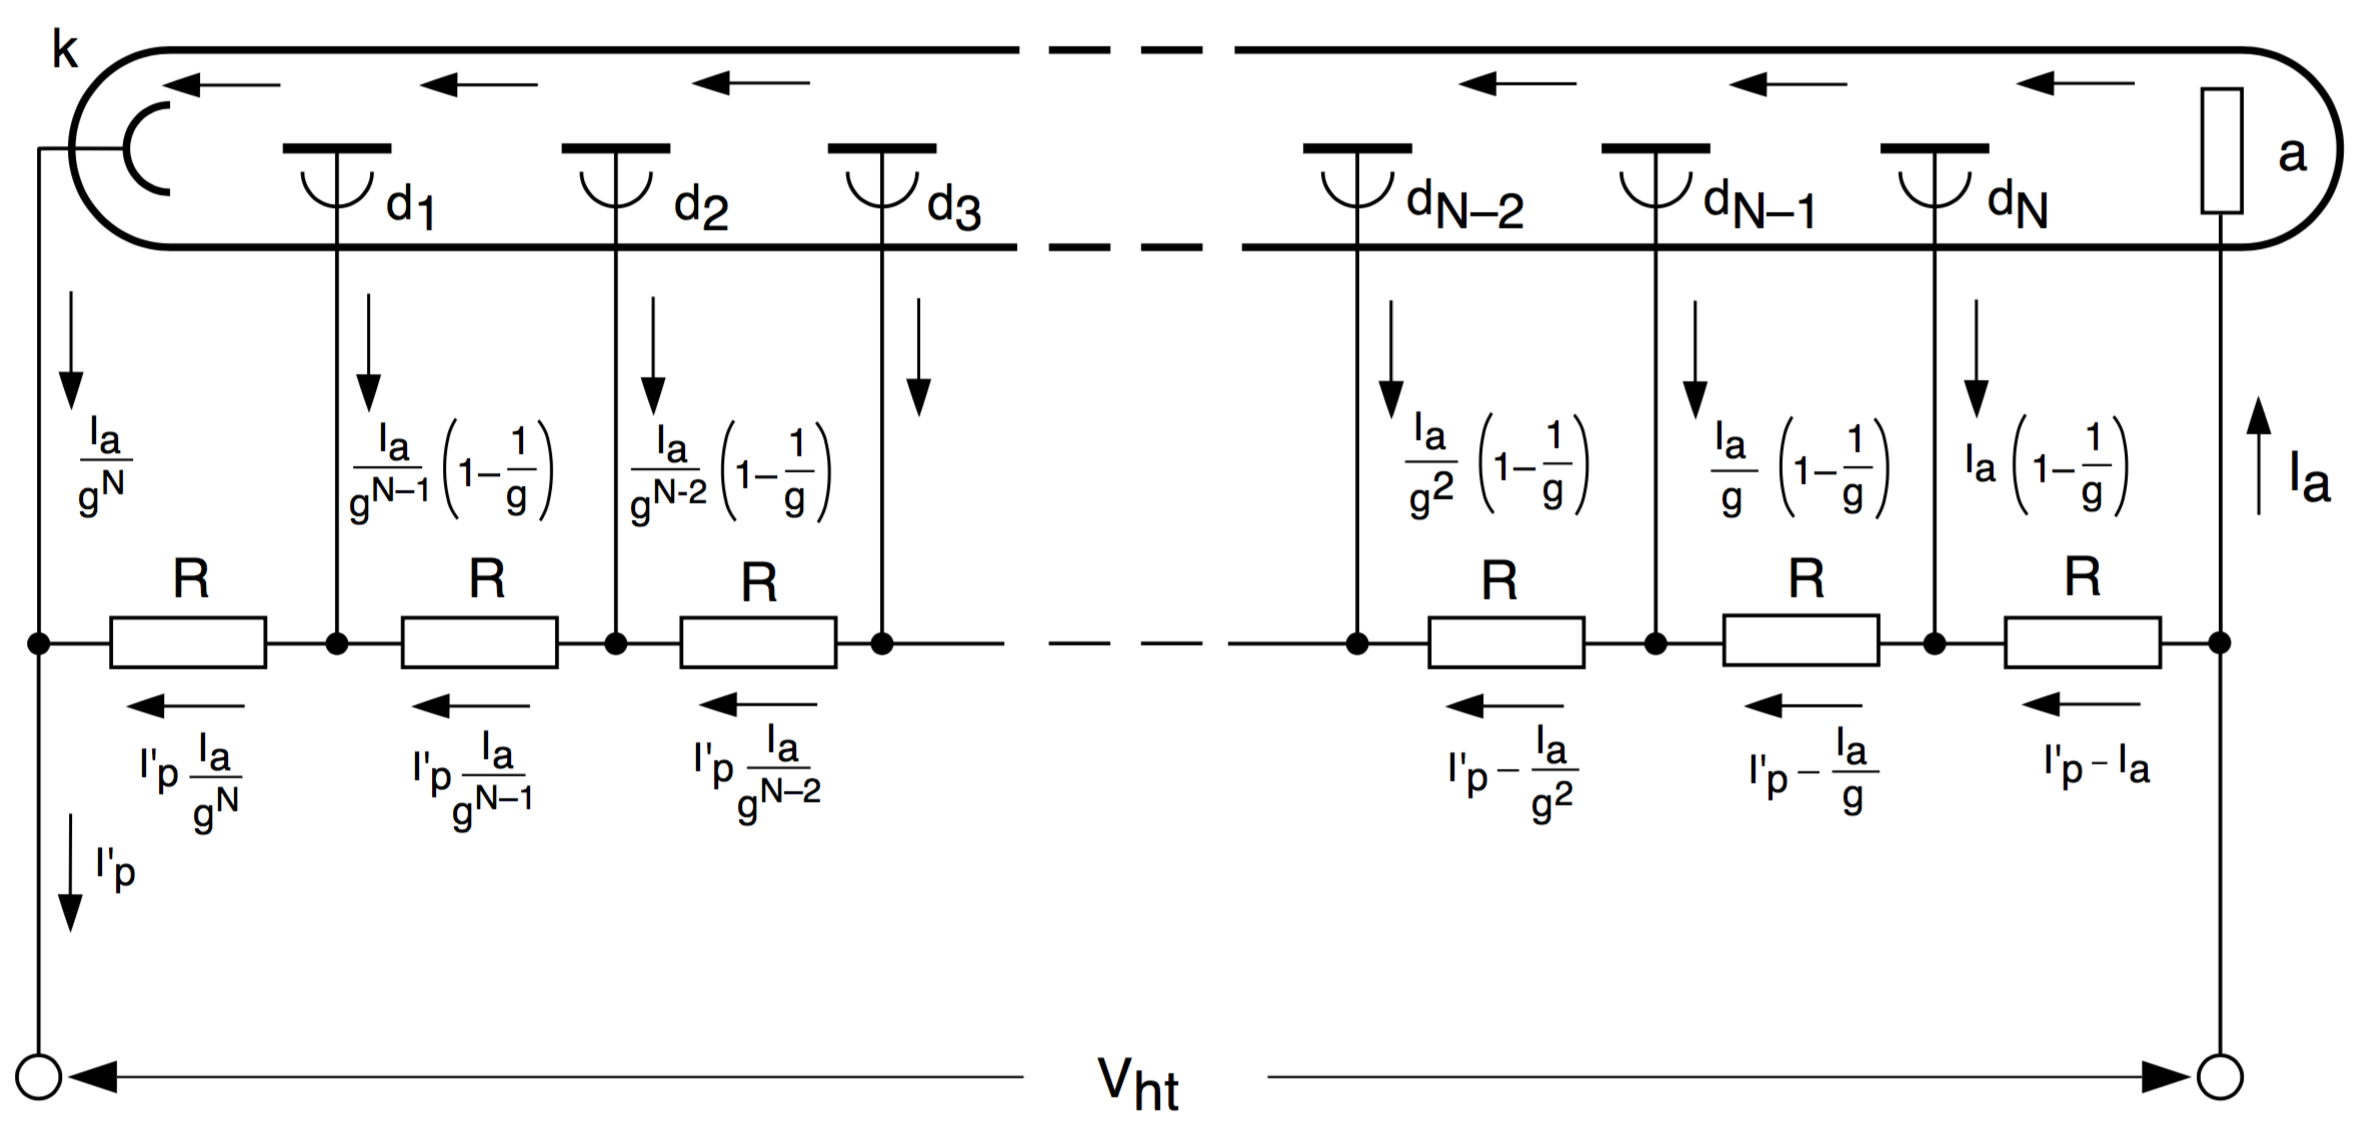
\includegraphics[width=0.8\textwidth]{chap/dynamic_range/fig/pmt_current_distribution_photonics.png}
	\caption{PMT工作时的电流分布图}
	\label{fig:dynamic_range:current_distribution}
\end{figure}
令PMT的打拿极总数为$N$,阳极的信号电流为$I_a$,分压器电流为$I'_p$以及极间增益系数为$g$,则整个PMT工作电路的电流分布如图~\ref{fig:dynamic_range:current_distribution}所示。
其中,第$n$个打拿极引出的电流信号可以表示为
\begin{equation}
	I_{dn} = \frac{I_a}{g^{N-n}}(1-\frac{1}{g})
	\label{eq:dynamic_range:dynode_current}
\end{equation}
而阴极电流为$I_a/g^N$,结合公式\ref{eq:dynamic_range:dynode_current},可以推得第$n$个打拿极的增益系数$G_{dn}$为
\begin{equation}
	G_{dn} = g^n(1-\frac{1}{g})
	\label{eq:dynamic_range:dynode_gain}
\end{equation}
依据公式\ref{eq:dynamic_range:dynode_gain},同时结合之前得到的平均光电子数$N_{pes}$和极间增益系数$g$,可以估算出各打拿极的增益以及输出信号所带的电荷量。
最终,R4443的第8打拿极(Dy8)被选择为高增益通道,用于覆盖动态范围需求的低半段;R4443的第5打拿极(Dy5)被选择为低增益通道,用于覆盖动态范围需求的高半段。
Dy8的典型增益为$4.71\times10^4$,对于\SI{1}{MIP}的输出信号电荷量约为\SI{362}{\femto\coulomb}。
虽然这个数值比设计值\SI{300}{\femto\coulomb}略大,但通过调节工作电压可以消除该差异。
而在标准工作电压下,Dy5和Dy8间的典型相对增益值约为63。
这个值略大于设计值35,但它满足我们的设计要求,而且也可以改变工作电压对其进行调节。

\subsection{分压器电路的设计}
\label{sec:dynamic_range:hv_divider}
光电倍增管的分压器具有两个基本功能:1.给PMT提供工作电压,并按一定的比例合理分配各光阴极、打拿极和阳极间的电势差;2.电流信号引出。
一般的分压器电路都是从阳极引出电流信号,不能够满足PSD的读出需求,因此我们对R4443的分压器电路进行了重新设计,如图\ref{fig:dynamic_range:divider}所示。
其中,打拿极9、打拿极10与阳极串联在一起,在工作中并不使用;而打拿极5和打拿极8处各增加了一段引出电路,用于电流信号的引出。
\begin{figure}[htbp]
	\centering
	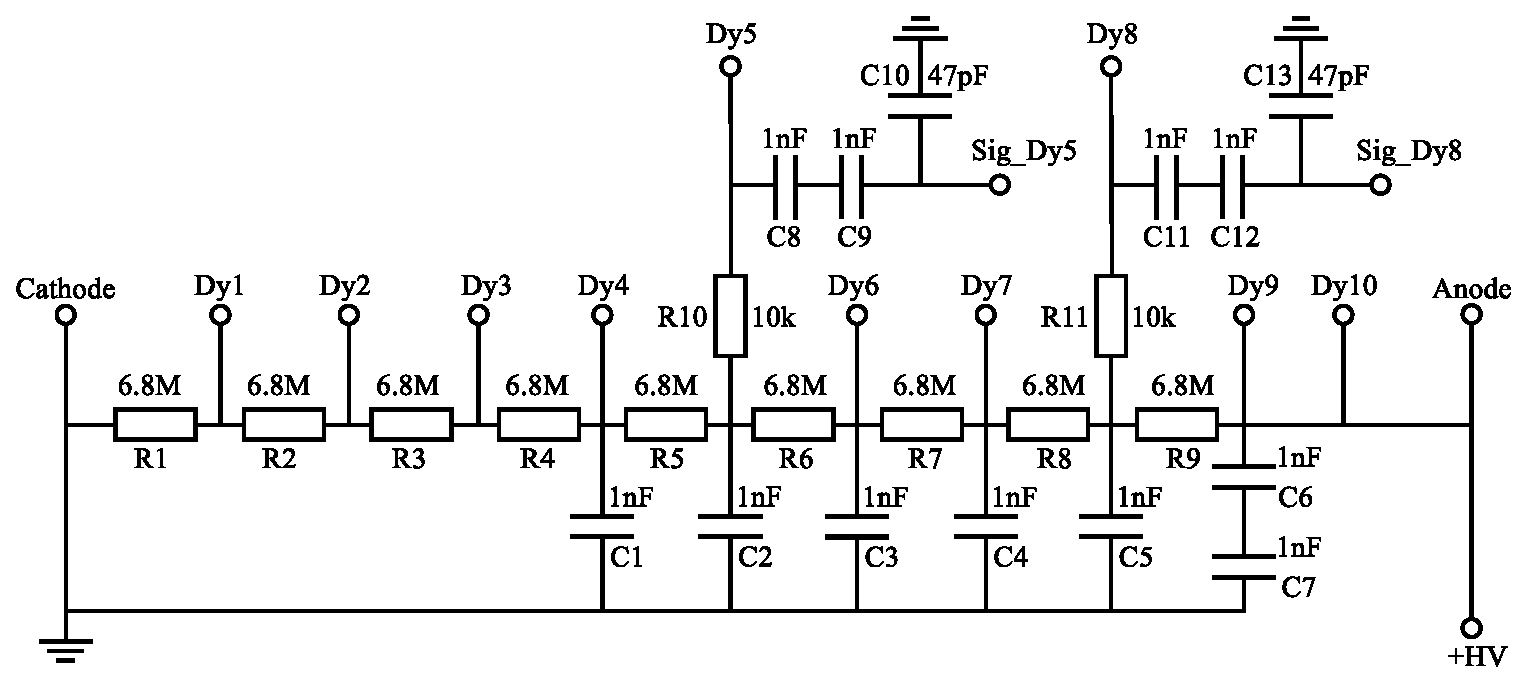
\includegraphics[width=0.95\textwidth]{chap/dynamic_range/fig/divider.eps}
	\caption{PSD的分压器电路原理图}
	\label{fig:dynamic_range:divider}
\end{figure}

为了尽量降低光阴极的输入噪声,PSD分压器的光阴极端(图中的Cathode)接地,并使用正电压供电。
另外,在PSD的工作范围内,R4443的输入光强并不算大,而R4443内部的极间空间电荷效应也并不显著。
因此,为了减少元器件种类和提高可靠性,该分压器采用均匀的极间电压分布,即$R_1 \sim R_9$的阻值相等。
而且,打拿极4到打拿极9间并联了一系列高压电容$C_1 \sim C_7$,用于在大输入光强时补偿后面几个打拿极间的分压器电流,保证了极间电压的稳定。
由于极间的增益系数取决于极间电压的大小,这也保证了PMT的增益线性。

打拿极5和打拿极8的引出电路采用相同的设计。
阻尼电阻$R_{10}/R_{11}$和电容$C_{10}/C_{13}$可以改善输出电流信号的波形。
由于分压器电路采用正高压供电,引出电路需要使用隔直电容来保护后面低压直流供电的FEE电路。
隔直电容采用冗余设计,即由两个电容串联组成(即打拿极5支路的$C_8/C_9$和打拿极8支路的$C_{11}/C_{12}$)。
这样,在一个隔直电容失效后,另一个隔直电容还能继续保护后续电路,提高了系统可靠性和安全性。

TODO:\emph{双绞线,实物图,电路板设计}

\section{大动态范围读出方案的原理验证}
\label{sec:dynamic_range:verification}
为了验证上述大动态范围读出方案设计的合理性,我们对PSD的一个探测器单元模块进行了详细的测试,分别是地面宇宙线的测试和相对论重离子$^{40}Ar$的束流测试。
测试结果显示,该读出方案完全满足PSD大动态范围的需求。
本节将对这些测试进行简单介绍,并给出测试结果。
由于PSD探测单元模块两端得到了相似的测试结果,为了叙述方便,下文中只对其中一端的结果进行了介绍。

TODO:\emph{探测器单元模块实物图}
% \subsection{LED的测试}
% \label{sec:dynamic_range:led}

\subsection{宇宙线测试}
\label{sec:dynamic_range:cosmic_ray}
到达地面的宇宙线主要由原初宇宙线和地球大气层反应产生的次级$\mu$子构成。
宇宙线$\mu$子是带一个电荷的最小电离粒子,经常被用于研究粒子探测器的MIP响应和在地面对探测器进行刻度。

图~\ref{fig:dynamic_range:cosmic_test}给出了PSD探测单元模块进行宇宙线测试的装置示意图。
其中,S1和S2是两个大小为$\SI{10}{mm} \times \SI{10}{mm} \times \SI{10}{mm}$的塑料闪烁体探测器。
它们分别放置在PSD探测单元模块单元条的上部和下部,其中心连线与被测单元条相互垂直,用于标识垂直入射的宇宙线事例。
S1和S2被固定在一个可以沿单元条方向移动的支撑台上,从而可以研究单元条不同位置处的MIP响应。
测试时,S1和S2的信号相与后作为触发信号输入到PSD的DAQ获取板中(详见第\ref{ch:description}章;DAQ板再把触发信号分发到FEE板,时FEE对此次事件进行处理,并将处理结果上传到DAQ板;最终,数据被DAQ收集、整理并上传到计算机进行保存。
\begin{figure}[htbp]
	\centering
	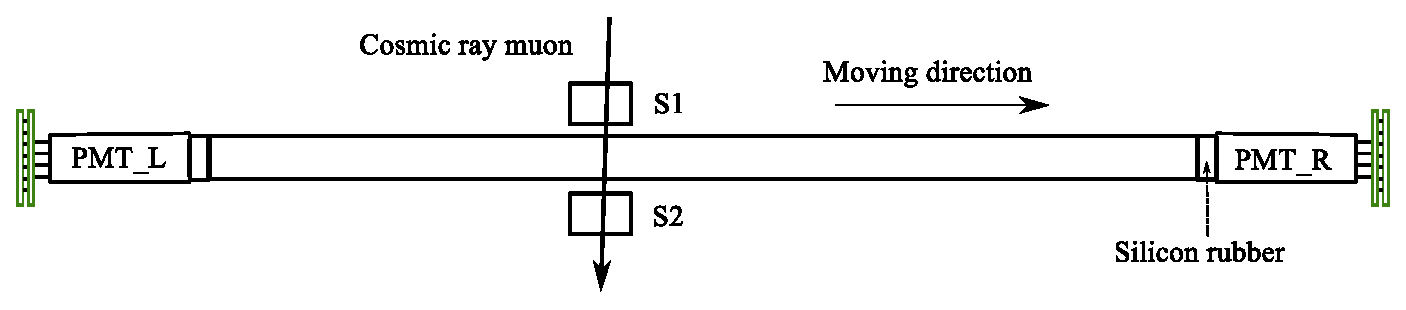
\includegraphics[width=0.95\textwidth]{chap/dynamic_range/fig/cosmic_test.eps}
	\caption{PSD探测单元模块的宇宙线测试}
	\label{fig:dynamic_range:cosmic_test}
\end{figure}

S1和S2首先移动到单元条的中心位置处,考察PSD探测单元模块的1MIP的能量响应。
正式测试前进行了若干次预备测试,每次测试使用不同的PMT工作电压以考察MIP峰位的移动。
最终,该探测单元模块的分压器电压确定为870V。
在该工作电压下,Dy8通道得到的MIP原始谱如图~\ref{fig:dynamic_range:mip}所示(蓝色部分)。
上图同时给出了该测量通道的基线原始谱(黑色部分),可以看到MIP峰和基线噪声可以很好地区分开来。
\begin{figure}[htbp]
	\centering
	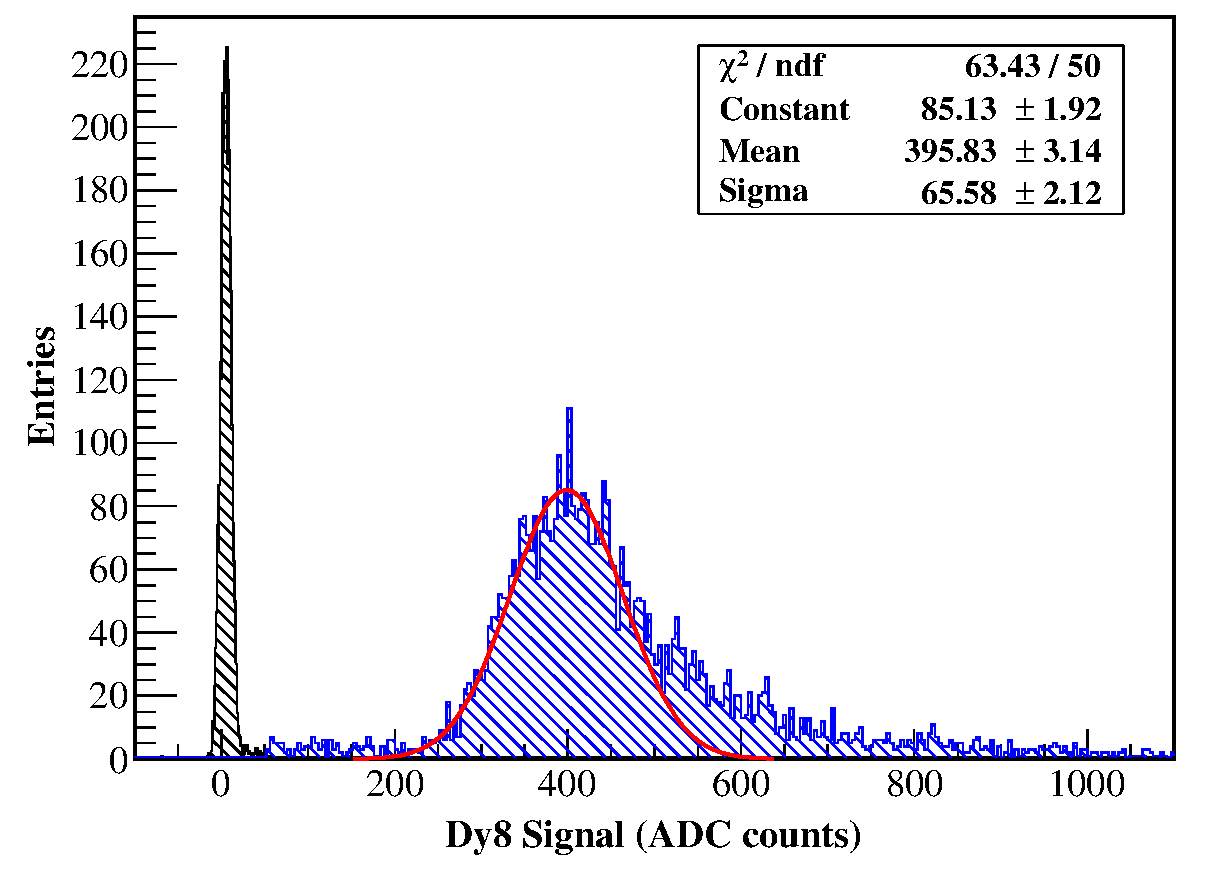
\includegraphics[width=0.6\textwidth]{chap/dynamic_range/fig/mip.eps}
	\caption{PSD单元条中间位置处的MIP响应。横轴为ADC道数,纵轴为事例数}
	\label{fig:dynamic_range:mip}
\end{figure}
MIP原始谱符合朗道分布,使用高斯分布对MIP峰的前半部分进行拟合,可以得到其最可几值(Most Probable Value,简称MPV)为395.8。
同样使用高斯分布拟合,可以得到该通道的基线噪声$\sigma$值为5.8。
以$5\sigma$为界限,则该探测单元模块动态范围下限可以计算为$5\cdot5.8/398.5\simeq\SI{0.0073}{MIPs}$。
这个值小于\SI{0.1}{MIPs},因此满足我们的设计要求。
上述测量结果都以ADC道数为单位,为了得到该通道所覆盖的动态范围上限,需要将ADC道数传化为电荷量。
利用FEE自带的电荷刻度模块,得到该测量通道的刻度参数值为\SI{1.082}{\per\femto\coulomb}。
结合FEE测量通道的有线线性范围(\SI{12}{\pico\coulomb}),则该单元模块Dy8通道的动态范围上限为$12000\cdot 1.082/395.8 \simeq \SI{32.6}{MIPs}$。

从单元条中心位置出发,将S1和S2沿着单元条以\SI{10}{cm}的间隔向左右两边移动,以考察单元条不同位置处的MIP响应。
将每个位置点处MIP谱的MPV值提取出来,就得到了MPV随击中位置的变化,如图\ref{fig:dynamic_range:attenuation}所示。
\begin{figure}[htbp]
	\centering
	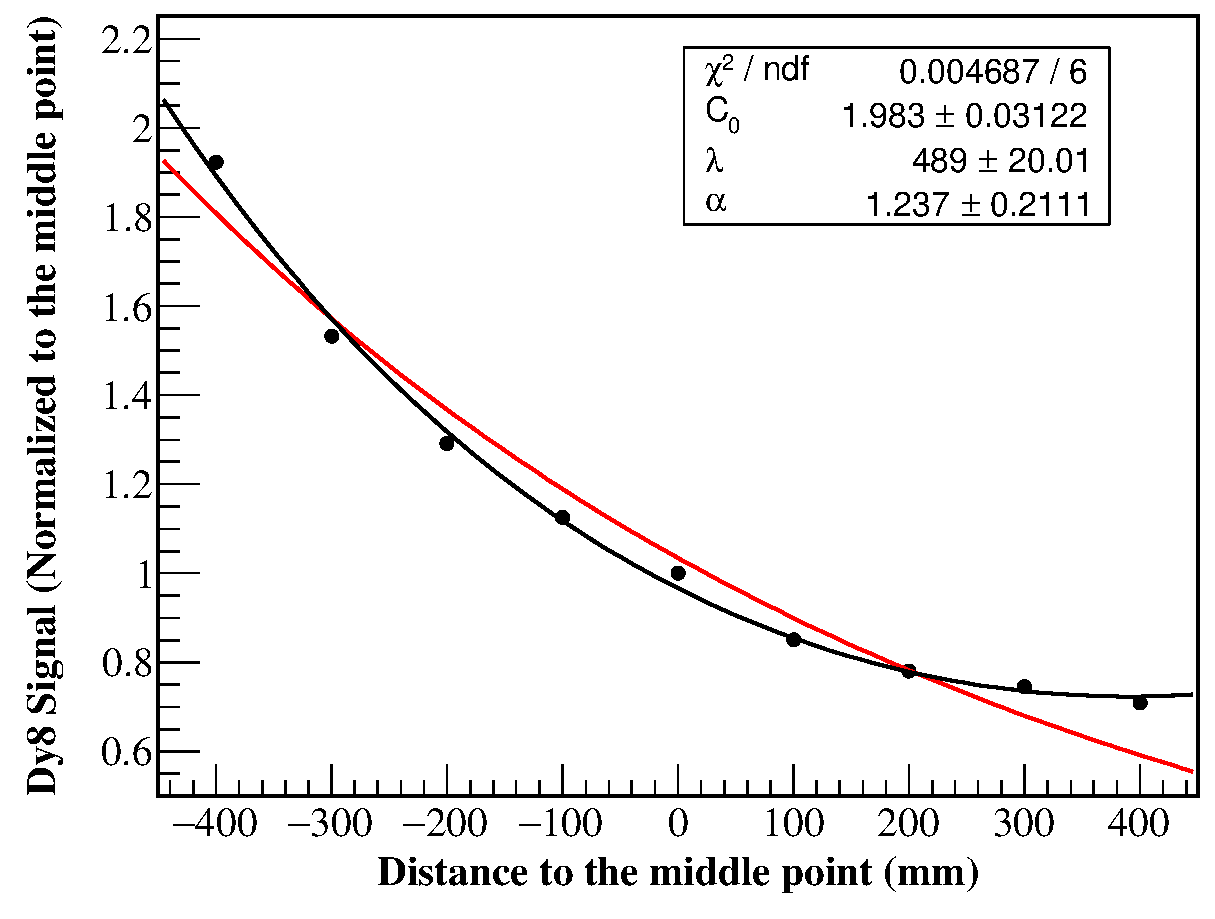
\includegraphics[width=0.6\textwidth]{chap/dynamic_range/fig/atten_right.eps}
	\caption{PSD单元条的光衰减曲线。横轴是以单元条中心为零点的位置坐标,横轴是相对中心位置归一的MPV值。}
	\label{fig:dynamic_range:attenuation}
\end{figure}
由于MPV值正比于平均光输出,图\ref{fig:dynamic_range:attenuation}同时也反应了单元条的光传输衰减效应。
\begin{equation}
\label{eq:attenuation}
A(x)=C_0(e^{-x/\lambda} + \alpha e^{-(2L-x)/\lambda})
\end{equation}


\begin{figure}[htbp]
	\centering
	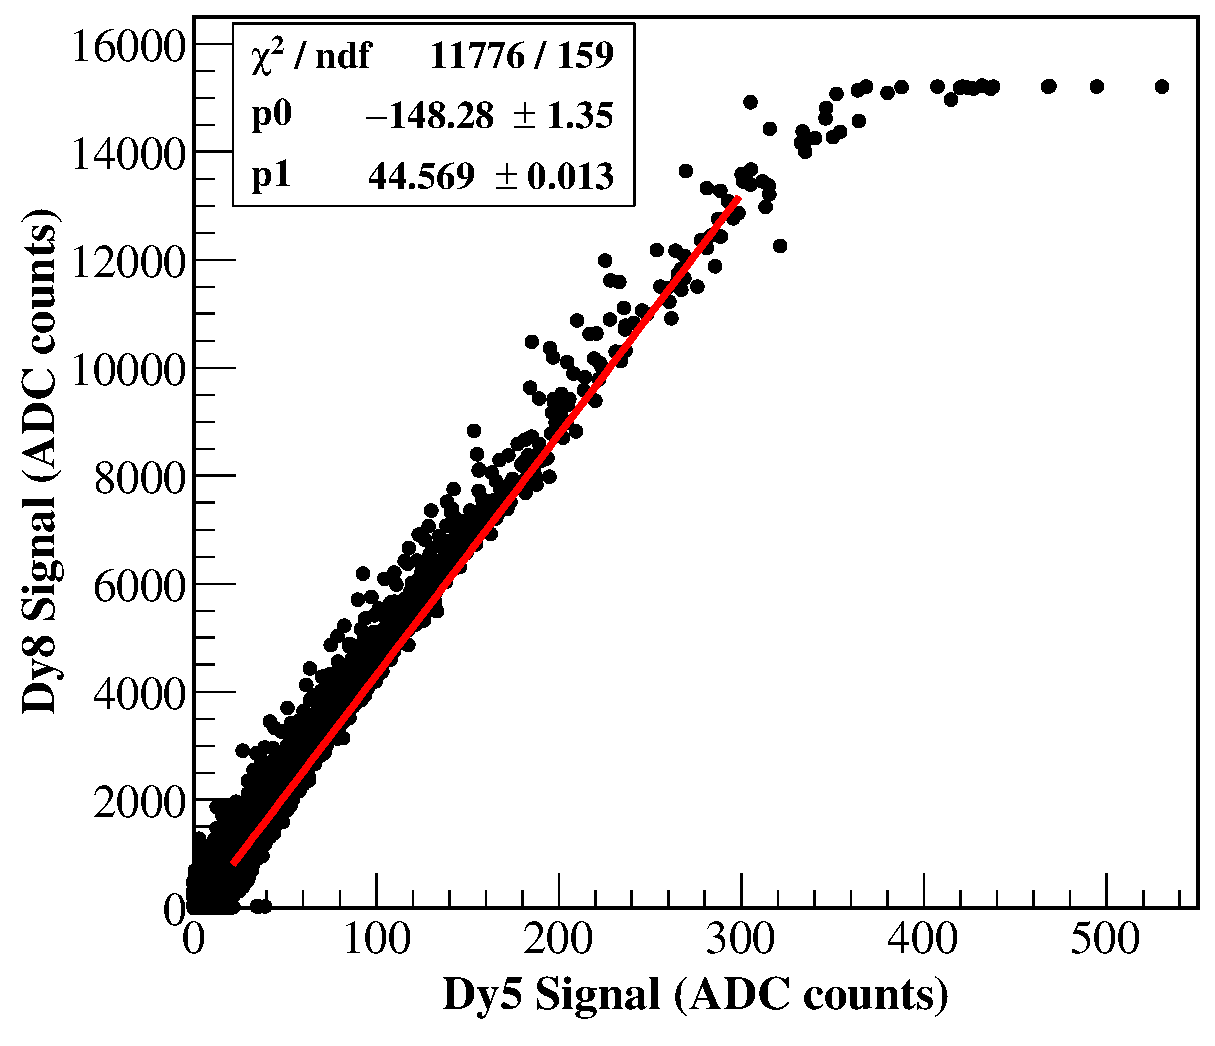
\includegraphics[width=0.6\textwidth]{chap/dynamic_range/fig/dy58.eps}
	\caption{Dy8与Dy5通道的ADC道数关联谱}
	\label{fig:dynamic_range:dy58}
\end{figure}

\subsection{相对论$^{40}Ar$束测试}
\label{sec:dynamic_range:ion_beam}

\begin{figure}[!htbp]
	\centering
	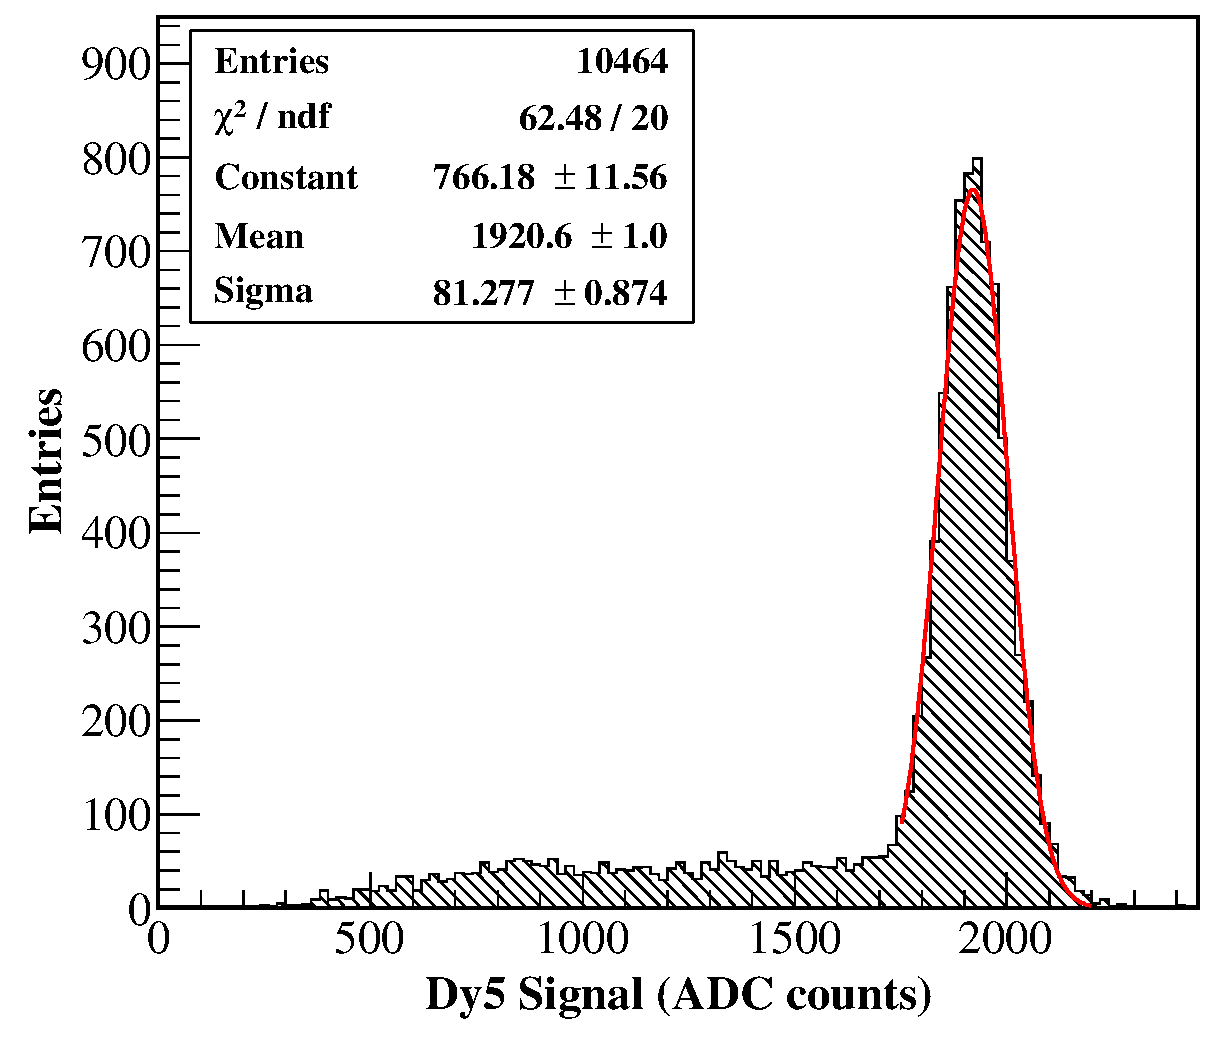
\includegraphics[width=0.6\textwidth]{chap/dynamic_range/fig/Ar.eps}
	\caption{$^{40}Ar$击中PSD单元条中间位置处的ADC原始谱}
	\label{fig:dynamic_range:Ar}
\end{figure}